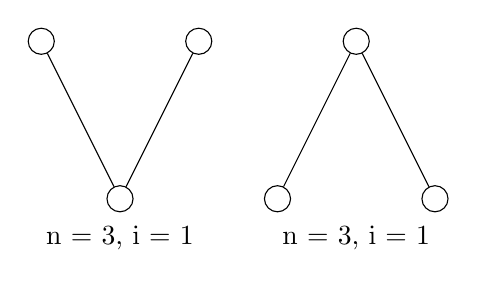
\begin{tikzpicture}
  \node[circle,draw=black] (A1) at (1, 0) {};
  \node[circle,draw=black] (A2) at (0, 2) {};
  \node[circle,draw=black] (A3) at (2, 2) {};

  \draw (A1) -- (A2) node {};
  \draw (A1) -- (A3) node {};
  \node (AL) at (1, -0.5) {n = 3, i = 1};


  \node[circle,draw=black] (B1) at (3 + 1, 2) {};
  \node[circle,draw=black] (B2) at (3 + 0, 0) {};
  \node[circle,draw=black] (B3) at (3 + 2, 0) {};

  \draw (B1) -- (B2) node {};
  \draw (B1) -- (B3) node {};
  \node (BL) at (3 + 1, -0.5) {n = 3, i = 1};
\end{tikzpicture}